%\documentclass[a4paper]{article}
\documentclass[final]{ua-thesis}
%% Language and font encodings
\usepackage{gb4e}
\noautomath
\usepackage{natbib}
\usepackage[english]{babel}
\usepackage[utf8x]{inputenc}
\usepackage[T1]{fontenc}

%% Sets page size and margins
%\usepackage[a4paper,top=3cm,bottom=2cm,left=3cm,right=3cm,marginparwidth=1.75cm]{geometry}

%% Useful packages
\usepackage{amsmath}
\usepackage{graphicx}
\usepackage[colorinlistoftodos]{todonotes}
\usepackage[colorlinks=true, allcolors=blue]{hyperref}
\usepackage{fixltx2e}
\usepackage{titlesec}
\usepackage{rotating}
\usepackage{qtree}
\usepackage{fixltx2e}

\usepackage{url}
\usepackage{amsmath}
\usepackage{graphicx}
\usepackage{color}
\usepackage{epic,ecltree}
\usepackage{eclbip}
\usepackage{multicol}
\usepackage{algorithmic}
\usepackage{algorithm}
\renewcommand{\algorithmicrequire}{\textbf{Input:}}
\renewcommand{\algorithmicensure}{\textbf{Output:}}
\renewcommand{\algorithmiccomment}[1]{// {\em #1}}

\definecolor{darkblue}{rgb}{0,0,0.8}
\definecolor{darkgreen}{rgb}{0,0.8,0}
\definecolor{reddishgreen}{rgb}{0.4,0.6,0}
\definecolor{purple}{rgb}{0.6,0,0.6}
\definecolor{red}{rgb}{1,0,0}

\newcommand{\example}[1]{\textcolor{darkblue}{\rm #1}}
\newcommand{\maths}[1]{\textcolor{purple}{#1}}
\newcommand{\reference}[1]{\vspace{-2mm}\begin{flushright}\textcolor{purple}{\tiny [from #1]}\end{flushright}\vspace{-7mm}}


\setcounter{secnumdepth}{4}

% \titleformat{\paragraph}
% {\normalfont\normalsize\bfseries}{\theparagraph}{1em}{}
% \titlespacing*{\paragraph}
% {0pt}{3.25ex plus 1ex minus .2ex}{1.5ex plus .2ex}
\usepackage{Sweave}

\newcommand*{\myfont}{\fontfamily{ccr}\selectfont}
%the newcommand change the selected word into 'ccr' font
%e.g. \begin{myfont} multi-bleu.perl \end{myfont}

\title{Developing Linguistically Informed Neural Net Machine Translation Systems}
\author{Yuan-Lu Chen}

\begin{document}
\Sconcordance{concordance:fakeMaster.tex:fakeMaster.Rnw:%
1 33 1}
\Sconcordance{concordance:fakeMaster.tex:./fakeCake.Rnw:ofs 34:%
1 148 1}
\Sconcordance{concordance:fakeMaster.tex:./GLOSS_table.Rnw:ofs 183:%
1 1 17 23 0}
\Sconcordance{concordance:fakeMaster.tex:./fakeCake.Rnw:ofs 208:%
151 20 1}
\Sconcordance{concordance:fakeMaster.tex:./ParaPart_table.Rnw:ofs 229:%
1 1 17 23 0}
\Sconcordance{concordance:fakeMaster.tex:./fakeCake.Rnw:ofs 254:%
173 5 1}
\Sconcordance{concordance:fakeMaster.tex:./Para_table.Rnw:ofs 260:%
1 1 17 23 0}
\Sconcordance{concordance:fakeMaster.tex:./fakeCake.Rnw:ofs 285:%
180 2 1}
\Sconcordance{concordance:fakeMaster.tex:./interleavingGdGLOSS_table.Rnw:ofs 288:%
1 1 17 23 0}
\Sconcordance{concordance:fakeMaster.tex:./fakeCake.Rnw:ofs 313:%
184 3 1}
\Sconcordance{concordance:fakeMaster.tex:./concate_table.Rnw:ofs 317:%
1 1 17 23 0}
\Sconcordance{concordance:fakeMaster.tex:./fakeCake.Rnw:ofs 342:%
189 3 1}
\Sconcordance{concordance:fakeMaster.tex:./ReplacingGaelic_table.Rnw:ofs 346:%
1 1 17 23 0}
\Sconcordance{concordance:fakeMaster.tex:./fakeCake.Rnw:ofs 371:%
194 3 1}
\Sconcordance{concordance:fakeMaster.tex:./ReplacingGLOSS_table.Rnw:ofs 375:%
1 1 17 23 0}
\Sconcordance{concordance:fakeMaster.tex:./fakeCake.Rnw:ofs 400:%
199 3 1 1 9 23 0 1 2 9 1}
\Sconcordance{concordance:fakeMaster.tex:fakeMaster.Rnw:ofs 438:%
36 5 1}


\maketitle

\chapter{Introduction}
\label{chap:Introduction}

Key information to be included:
\begin{enumerate}
\item outline/organization of the dissertation 
\item Arguments to be made in the dissertation: 
	\begin{enumerate}
	\item To understand language, NLP and Linguistics should work together.
    \item  Gloss is the right `lingua franca' for the two fields.
    \item Linguistics helps NLP.
    \item NLP helps linguistics. 
	\end{enumerate}
\end{enumerate}
\chapter{What are glosses? Why are them golden representations of meanings?}
\label{chap:gloss}

\section{Key Points of The Chapter}
	\begin{enumerate}
	\item Target Audience: CS people
	\item main points:
		\begin{enumerate}
    	\item summary of the Leipzig Glossing Rules \citep{bickel2008leipzig}.  
		\item glossing is the initial processing of the data guided by some specific syntax theory. 
    	\item Glosses contain morphology information (with examples); glosses disambiguate homographs (with many examples); gloss also provide some parsing information because some glosses are determined by structural/constituency context (with examples).       
		\end{enumerate}
 
	\end{enumerate}

\section{Introduction: What are Glosses}

Interlinear Glossed Text (IGT) is widely used in linguistic studies. (\ref{gloss_eg}) is an example of Scottish Gaelic IGT.
\begin{exe}  
\ex\label{gloss_eg} \gll    Tha a athair nas sine na a mh\`athair.\\  
            be.pres 3sm.poss father comp old.cmpr comp 3sm.poss mother
\\  
    \glt    `His father is older than his mother.'  
\end{exe}

(summarize and exemplify the Leipzig Glossing Rules)


\section{The Golden Properties of Glosses}

A system of meaning representations is decomposed of three components: a) meanings, b) representations, and c) a mapping between meanings and representations. The most ideal meaning representation system should be built with one-meaning-to-one-representation mappings; in other words, a meaning is mapped to one and only one representation. Natural languages fail to do so, given that synonyms and ambiguous words/phrases are ubiquitous in natural languages. On the other hand, gloss provides a mapping that is close to this ideal one-to-one mapping. Thus gloss should a better representation in term of representing meanings. 

Theoretically, the claim that gloss representation is closer to the ideal one-to-one mapping than natural language representation is can be tested empirically. IF there were a set of special golden meta-linguistic semantic representations, which has the following property: each concept is mapped to one and one representation and each representation is mapped to one and one concept, then it is expected that each gold representation will map to more natural language words than gloss items, and each natural language word will map to more gold representations than gloss items. However, in practice, this is an impossible experiment to conduct, because there are no such golden representation\footnote{It would solve the puzzle of semantics if one should be able to build the set of special golden meta-linguistic semantic representations, and the mappings between the golden representations to natural languages.}. However, in spite of the impossibility of conducting statistical experiments, we may still use some examples to show the intuition that glosses are better representations than natural languages. The following sections describes how glosses cluster words with different forms but with the same meaning, and how glosses represent words with same form but with different meanings with different representations. 

\subsection{Glosses Cluster Different Words with the Same Meanings (Synonyms) Into a Single representation}
Gloss collapses words with different forms with the same meanings into a single gloss. In natural languages, the morphology of a word (i.e. the form of a word) may be sensitive to the phonological environments and changing into different forms. Consider the following the indefinite article in the English examples: 

\begin{exe}  
\ex \gll John ate \textbf{an} apple.\\
	John eat.past	\textbf{ART} apple\\
\ex \gll John ate \textbf{a} banana.\\
	John eat.past   \textbf{ART} banana\\
\end{exe}

In the above example, \textit{an} and \textit{a} have the identical meaning\footnote{Semantically, \textit{an} and \textit{a} are existential quantifiers, which declare that a member of a set exists in the world. In formal semantics, \textit{an} and \textit{a} may be defined as follows: $\exists\lambda P[P(x)]$. In the current example, \textit{apple} and \textit{banana} will instantiate $P$ in the formula, and the meanings will be `an apple exists' and `a banana exists'. \citet{kratzer1998semantics} would be a nice introduction for interested readers to see how linguists, specifically semanticians, define, decompose, and compose meanings of languages formally.}. 
In English, the same concept is realized as two representations, \textit{a} or \textit{an}, while in the gloss representation the one concept is neatly represented as \textit{ART}. 

Critically, synonyms like the English \textit{a} and \textit{an} commonly occur in many other natural languages if not in all languages. The definite article in the language of interest, Scottish Gaelic, is another example to show the noisiness of natural language representations. Consider the definite article in the following Gaelic examples. 

\begin{exe}  
\ex 
\gll tha mi a' sireadh \textbf{an} leabhair bhig ghuirm\\
be-PRES-IND 1S PROG searching-VN \textbf{ART} book-G small-G blue-G\\
\glt `I am looking for the small blue book' \citep[p. 29]{lamb2001scottish}

\ex 
\gll \textbf{am} fear m\`or\\
\textbf{ART} man big\\
\glt `a big man' \citep[p. 31]{lamb2001scottish}

\ex
\gll thuit \textbf{a'} chlach air cas mo mhn\`a\\
fall-PAST \textbf{ART} stone on foot 1S-POSS wife-G\\
\glt`the stone fell on my wife's foot' \citep[p. 30]{lamb2001scottish} 	

\ex
\gll doras \textbf{na} sgoile(adh) \\
door-N \textbf{ART} school-G \\
\glt `the door of the school' \citep[p. 29]{lamb2001scottish} 	

\ex 
\gll a chuir air d\`oigh \textbf{nan} \`airidhean a-muigh a rubh' Eubhal agus an oidhche seo \\
to put-INF on order \textbf{ART} sheilings out-LOC to point Eaval and ART night this \\
\glt `the girls big house' \citep[p. 100]{lamb2001scottish} 

\ex
\gll f\`eis \textbf{nam} b\`ard\\
festival \textbf{ART} poet.PL.GEN\\
\glt `festival of the poets' \citep[p. 107]{lamb2001scottish}

\end{exe}

The definite article in Scottish Gaelic may be realized as the following forms: as \textit{an}, \textit{am}, \textit{a'}, \textit{na}, \textit{nan} or \textit{nam}. The alternation is determined by the case, gender and number of noun phrase that it modifies, and additionally the phonological property of the word following it also changes the form of the definite article \citep{lamb2001scottish}. All these different realizations refer to the same concept, the definite article. Again, the gloss notation nicely clusters them together as \textit{ART}. 

In Mandarin Chinese, similar patterns are found. Consider classifiers in the following examples:

\begin{exe}
\ex \label{chinese_cl_eg}
\gll Yani mai-le \{\textbf{pi}/\textbf{*tou}\} ma , Lulu mai-le \{\textbf{*pi}/\textbf{tou}\} zhu.\\ 
Yani buy-PRF CL/CL horse , Lulu buy-PRF CL/CL\\
\glt `Yani bought a horse and Lulu bought a pig.' \citep[p. 136]{zhang2013classifier}
\end{exe}

In \citet{zhang2013classifier}, the classifier like \textit{pi} and \textit{tou} is a type of \textit{indivual classifier} which co-occurs with countable nouns, like \textit{ma}, `horse', and \textit{zhu}, `pig', and this type of classifier is the head of \textit{UNIT Phrase}. 
\textit{Pi} and \textit{tou} actually have the same semantics and the syntactic function; however, they are realized in different forms, specifically the form of which has to agree with the noun following it (i.e. \textit{pi} goes with \textit{ma}; \textit{tou} goes with \textit{zhu}). Here the gloss, \textit{CL}, unifies the two forms of the same meaning.    

In short, gloss collapses synonyms in natural languages. Learning the general distribution of the article and all its different forms is a challenge for the MT system, but the glossing information should make this easier.

\subsection{Glosses Distinguish Homographs' Different Meanings}

In natural languages, there are cases when a single form denotes to distinct concepts. Words with this properties are termed as homographs. Consider the word \textit{for} in following English examples:

\begin{exe}
\ex \label{for_eng}
	\begin{xlist}
	\ex \label{for_c}I intended \textbf{for} Jenny to be present.
	\ex \label{for_p}\textbf{For} Jenny, I intended to be present. \citep[p.306-307]{adger2003core}
	\end{xlist}
\end{exe}

\textit{For} in (\ref{for_c}) and (\ref{for_p}) has the same form but different meanings. Specifically, \textit{for} in (\ref{for_c}) is a complementizer with its part of speech being \textit{C}, and it heads the non-finite clause \textit{Jenn to be present}; on the other hand \textit{for} (\ref{for_p}) is a preposition, which takes the Determiner Phrase, \textit{Jenny}, as its benefactive argument.   

The Scottish Gaelic word \textit{a'} in the following examples also has different meanings.  

\begin{exe}  
\ex \label{a_prog}
\gll tha mi \textbf{a'} sireadh an leabhair bhig ghuirm.\\
be-PRES-IND 1S \textbf{PROG} searching-VN ART book-G small-G blue-G\\
\glt `I am looking for the small blue book.' \citep[p. 29]{lamb2001scottish}

\ex \label{a_det}
\gll thuit \textbf{a'} chlach air cas mo mhn\`a.\\
fall-PAST \textbf{ART} stone on foot 1S-POSS wife-G\\
\glt`the stone fell on my wife's foot.' \citep[p. 30]{lamb2001scottish} 	
\end{exe}

Critically \textit{a'} in (\ref{a_prog}) is a progressive aspect marker while in (\ref{a_det}) the some form denotes to definite article. Again, the semantic difference is preserved in the gloss representations but not in natural language words.  
The gloss data also provides hierarchical (non-linear) syntactic parsing information. 

\subsection{Glosses are Sensitive to Hierarchical Structures in Natural Language Sentences}

Before I introduce how gloss information is linked to hierarchical structures, it is necessary to emphasize the importance of hierarchical structures in natural languages. In this section, I will first review some linguistic arguments for why and how semantics and syntax of languages\footnote{When it turns to the sound aspect of languages, Phonetics is more about linear order, but Phonology is still sensitive to hierarchical structures just like syntax and semantics. } are all about hierarchical structures instead of linear word orders. Then I will link gloss to hierarchical structures.

It is well-argued in linguistics that the syntax and semantics of natural languages are determined by hierarchical structures instead of linear orders of words, and essentially it is the sensitivity of hierarchical structures that distinguishes human natural languages from other animal communications \citep{berwick2015only}.     

Semantics is determined by hierarchical structures instead of linear orders. \citet[p. 117]{berwick2015only} use the following simple example to demonstrate this property of natural languages:

\begin{exe}
\ex Instinctively birds that fly swim. 
\end{exe}

In the example above, \textit{instinctively} is linearly close to \textit{fly} than \textit{swim}; however, it unambiguously modifies \textit{swim} instead of \textit{fly}. The reason for this is the hierarchical structures \citep[p. 117]{berwick2015only}:

\begin{exe}
\ex \label{tree}
\Tree [Instinctively [ [  birds   [  that   fly  ]  ]  swim  ] ]
\end{exe}

In (\ref{tree}) it is shown that \textit{fly} is more embedded than \textit{swim}, and thus it is hierarchically further away from \textit{instinctively}. So, \textit{instinctively} can only modify \textit{swim} instead of \textit{fly}.

Syntax is also all about hierarchical structures. Consider the following sentence:

\begin{exe}
\ex 
	\begin{xlist}
	\ex \label{aux_inver1} Birds that can\textsubscript{1} fly can\textsubscript{2} swim. 
	\ex \label{aux_inver2} *Can\textsubscript{1} birds that  fly can\textsubscript{2} swim? 
	\ex \label{aux_inver3} Can\textsubscript{2} birds that can\textsubscript{1} fly  swim? 
	\end{xlist}
\end{exe}

(\ref{aux_inver1}) is a declarative sentence. To derive an interrogative sentence from it, the auxiliary needs to be moved; however only \textit{can\textsubscript{2}} can be moved but not \textit{can\textsubscript{1}} even \textit{can\textsubscript{1}} is linearly close to the sentence initial position. Again, it is all because of the hierarchical structures. \textit{can\textsubscript{2}} is in the matrix clause while \textit{can\textsubscript{1}} is in the embedded relative clause.  

Word order and linearizion are just epiphenomena from the perspective of theoretical syntax and semantics. They are inevitable externalization of language because we are living in a world of linear time and space. To put this argument in another way, if externalization should be the primary nature of language, we should expect that some natural human languages should have manipulated the linear order of words in a sentence to express different meanings, because linear order is the externalization of language. However, this is not the case. No language exploits linear order, and instead universally language uses hierarchical structures, which is more difficult to be externalized than linear order. \citet{chomsky2006language} uses the following examples to illustrate this point.

\begin{exe}
\ex
	\begin{xlist}
	\ex\label{c1} Smart eagles can swim.
	\ex\label{c2} *Eagles smart can swim?
	\ex\label{c3} Can smart eagles swim?
	\end{xlist}
\end{exe}

(\ref{c1}) is a declarative sentence. (\ref{c2}) tries to swap the first two words to derive an interrogative sentence, and fails. (\ref{c3}) is the real interrogative sentence in natural languages. If externalization and communication are the primary nature of language, it is expected (\ref{c2}) to be a common pattern in languages, because (\ref{c2}) exploits linear order, which is the externalization of language and the linear order serves the communication purpose just fine given that humans' cognition system is able to tell the difference between (\ref{c1}) and (\ref{c2}). However, the pattern in (\ref{c2}) is not found in any human language; instead, (\ref{c3}) is used, which uses hierarchical structure relations. In term of externalization, (\ref{c2}) is more economical than (\ref{c3}) given that (\ref{c2}) only moves two positions of words while (\ref{c3}) moves three positions of words. Again, if externalization and communication are the primary nature of language, language should have evolved the pattern of (\ref{c2}). Based on the fact that no language exploits linear order, it is argued that language externalization and communication in particular are accessory.   

Glosses are also sensitive to the internal hierarchical structures or constituency of sentences. Consider the following examples, modified from \ref{for_eng}:

\begin{exe}
\ex
For as \textit{complementizer}
	\begin{xlist}
	\ex I intended \textbf{for} [Jenny] to be present.
	\ex I intended \textbf{for} [the girl] to be present.
	\ex I intended \textbf{for} [the little girl] to be present.
	\ex I intended \textbf{for} [the little girl who wants to eat some ice scream] to be present. 
	\end{xlist}
\ex
For as \textit{preposition}
	\begin{xlist}
	\ex \textbf{For} [Jenny], I intended to be present. 
	\ex \textbf{For} [the girl], I intended to be present. 
	\ex \textbf{For} [the little girl], I intended to be present. 
	\ex \textbf{For} [the little girl who wants to eat some ice scream], I intended to be present. 
	\end{xlist}
\end{exe}

Linear length of the argument of \textit{for} (i.e. the sequences in the square brackets) does not have any effect in determining what the gloss is, and instead it is the hierarchical structures that determines what the gloss is. 


\section{Conclusion: What is a Gloss Line?}  
A gloss line is an artificial sentence using the purified `gloss words', a meaning representation with which one meaning is mapped to one and only one representation. It is a useful and widely used annotation algorithm that requires linguistic knowledge. Given the properties of gloss data, it can be a very useful data for machine translation. Moreover, gloss data is widely used in linguistics literature, so data is already out there and all we need is to clean the data.  
In chapter \ref{chap:cake} and \ref{chap:cake2} I will report machine translation experiments using gloss data.  

% section conclusion (end)
\chapter{Description of the Scottish Gaelic Interlinear Glossed Text Corpus}
\label{chap:Corpus}

	\begin{enumerate}
    \item Original goal of the corpus: a bank of examples of specific syntactic patterns for syntacticians.  
	\item Description of UA Celtic Group's Scottish Gaelic documentation project\\
	The corpus has 8,367 Gaelic sentences, and in term of words, it has 52,778 Gaelic words/glosses. The data of the corpus is from two different sources: fieldwork and data elicitation. 
    \item Collection of interlinear glossed text data used in syntax paper/dissertations AND language documentation
    \item Auto-glosser and literature on auto-glosser
	\end{enumerate}
\chapter{A Gental Introduction of Machine Learning and Machine Translation}
\label{chap:MT}

	\begin{enumerate}
	\item General review of supervised Machine learning \citep{kotsiantis2007supervised}: The goal is provide a high level of understanding of what machine learning is. Machine Learning is to learn from EXAMPLES/SAMPLES. For example, to define the meaning of `dog', instead of giving all the definable features of `dog', we feed the machine with as many as possible of information of entities of dogs that we have access. Montague Semantics is actually a variant of ML, within which `dog' is defined as `the set of all the dog that exists in the current world.'. As such, Montague Semantics is Machine Learning, because instead of defining 'dog' with certain arbitrary rules (+/- FEATURE), it says 'all the dog entities in the current world'. Definition by samples/examples not by rules.    
	\item Literature on machine translation: from statistical machine translation \citep{koehn2009statistical} to neural machine translation \citep{cho2014learning,cho2014properties,bahdanau2014neural,Koehn_NMT2017}. (Target audience: linguists)
	\end{enumerate}
 
\section{Neural Net Machine Translation}\label{neural_MT}
Introduction of Neural Net Machine Translation
\chapter{Building Translation Systems using Interlinear Glossed Text}
\label{chap:cake}

(

\textbf{Assuming that in the previous chapters the following points are addressed already:}
\begin{itemize}
\item The nature of glosses has been well-explained  (Target audience: CS people without any formal linguistics background):
	\begin{itemize}
	\item What glosses are: A basic intro of interlinear gloss for non-linguists
   \item The golden nature of glosses (encodes NON-LINEAR syntax (i.e. structure parse) and semantics information)
   \item The potential of gloss:	
		\begin{itemize}
		\item potential: providing disambiguation, labeling important grammar morphemes in the source language, providing morphological analysis, providing one-to-many and many-to-one relations of source tokens and target tokens. 
		\end{itemize}
	\end{itemize}
\item A history of machine translation, and a non-mathy description of the methods of doing machine translation. (Target reader: theoretical linguists)
\end{itemize}

               
)


\section{Introduction}
The Innovation is to incorporate the gloss information of Interlinear Glossed Text data into machine translation.

In supervised machine learning models, two factors effects the performance of the trained systems \citep{kotsiantis2007supervised}: a.) the quality of the training data and b.) the choice of the features. The properties of the gloss data as described in chapter \ref{chap:gloss} make it a better training data than natural language data (Scottish Gaelic in the current case) for the following reasons. First, glosses are more purified than natural language words. The most ideal meaning representation system should be built with one-meaning-to-one-representation mappings; in other words, a meaning is mapped to one and only one representation. Natural languages fail to do so, given that synonyms and ambiguous words/phrases are ubiquitous in natural languages. Glosses provide this one-to-one mapping. Second, the gloss data provides hierarchical (non-linear) syntactic parsing information. To determine what the gloss of a word is, linguists have to look for hierarchical (non-linear) context information. See chapter \ref{chap:gloss} for the discussion on the golden properties of glosses.  

Therefore, theoretically incorporation of the gloss data should improve the translation systems. Specifically, I propose the following hypothesis:
\begin{exe} 
\ex \textbf{Gloss-helps hypothesis: the translation systems trained with the gloss data incorporated should outperform the systems trained with only Gaelic and English sentences pairs (i.e. without gloss data).}

The hypothesis can have two versions, strong and weak:
	\begin{xlist}
	\ex \label{strong_hy} Strong version: Gloss may replace the source natural language totally, and the system outperforms the system trained with source natural language to target language sentence pairs (i.e. the baseline systems).  
	\ex \label{weak_hy} Weak version: Gloss only increases the performance of the baseline systems, but cannot replace the source language.
	\end{xlist}
\end{exe}

The experiments reveal that replacing Gaelic words with glosses doesn't boost up the performance of the translation systems. Thus, the strong version (replacing-Gaelic-with gloss) of the Gloss-helps hypothesis is not attested. However, it is found that if the Gaelic data and the gloss data are combined in a specific way as the training data, the performance of the systems is improved significantly. 

This chapter describes the experiments conducted to test the Gloss-helps hypothesis and the results attest the weak version.
The rest of the chapter is organized as follows: Section \ref{relate_work} describes related works in the literature, Section \ref{sec:experimet_setting} describes the constant parameter settings across all the experiments, section \ref{gd_to_gl_to_en} tests the hypothesis in (\ref{strong_hy}), section \ref{gd_plus_gl_to_en} tests the hypothesis in (\ref{weak_hy}),and section 5 concludes the chapter. 

%%%%%%%%%%%%%%%%%%%%%%%%%%%%%%%%%%%%%%%%%%%%%%%%%%%%%%%%%%%%%%%%%%%%%%%%%%%%%%%%%%%%%%%%%
\section{Related Work}\label{relate_work}
Attempts to improve machine translation systems by incorporating explicit linguistic information are reported in the literature. Syntax information is known to be effective in improving statistical machine translation (SMT). The efforts of using syntax information even derive a special type of SMT, termed as syntax-based SMT \citep{williams2016syntax}. The same trend is also found in neural net machine translation. For example, \citet{sennrich2016linguistic} exploit the information of lemmas, part of tags, morphology of words, and dependency parses of sentences to improve MT systems. \citet{ccg_target_seq} incorporate the Categorial grammar parse tags of the target sequences.

%%%%%%%%%%%%%%%%%%%%%%%%%%%%%%%%%%%%%5

\section{Technical Settings of the Machine Translation Experiments}\label{sec:experimet_setting}
The experiments are conduced by using OpenNMT \citep{2017opennmt}, which implements the state-of-the-art neural net machine translation algorithms \citep{cho2014properties, cho2014learning, bahdanau2014neural}.
The following default hyper-parameter settings of OpenNMT\footnote{See their documentation for the complete default hyper-parameter settings: \url{http://opennmt.net/OpenNMT-py/}.} are used across all models so that the only independent variable is the type of the training data:
	\begin{itemize}
	\item Word vector size: 500\\
	In neural net machine translation, a word is represented as a vector. This hyper-parameter means that we are going to use vectors with 500 dimensions to represent words.
	\item Type of recurrent cell: Long Short Term Memory\\
	Long Short Term Memory recurrent neural net is a type of neural net that is suitable for sequence to sequence tasks.  
	\item Number of recurrent layers of the encoder and decoder: 2\\
	This hyper-parameter specifies that we are going to have two recurrent layers of the encoder and decoder. 
	\item Number of epochs: 13\\
	The training process of a neural net machine translation systems is done epoch by epoch. Each epoch is an iteration of training. Here 13 means that we are going to have 13 iterations of training and thus have 13 epochs. 
	\item Size of mini-batches: 64\\
	Training a neural net is to let the weights of the connections between the neurons fit the training samples. Theoretically, we may ask the net adjust the weights according all the samples all together at one time. However, in practice, this is not memory efficient, and will cause errors in the process of optimizing the weight parameters. So, instead, the samples are split into smaller mini-batches, and the neural net just updates its weights to make the most accurate predictions for a mini-batch at one time. This hyper-parameter specifies the size of a mini-batch. Actually finding the right mini-batch size is not a trivial but an important question in Deep Learning. See \citet{DBLP:journals/corr/KeskarMNST16} and \citet{DBLP:journals/corr/abs-1711-00489} for the experiments and discussions on the effects of the size of mini-batches. 
	\end{itemize}

The settings of the hyper-parameters do have effects on the performances of the trained models.
A common practice to find the optimal settings of the hyper-parameters is to hold out a subset of the training dataset as the developing dataset, then test the models on the developing data to see what settings are optimal, then merge the developing dataset and training dataset as a new training set, and then train on this new training set using the found optimal hyper-parameters.

However, given that finding the optimal settings of the hyper-parameters is not relevant to our research and causing unnecessary complications, the process of optimizing the settings of the hyper-parameters is not implemented, and I simply adopt OpenNMT's default settings. The employed settings of the hyper-parameters should be viewed as arbitrarily chosen, and there are room to tune the models for better performance. Critically, these settings are viewed as constants, so that we can focus on the effects of different treatments on the source sequences in the translation experiments.  We will leave the question of what hyper-parameters are optimal for our data for future research.

The data and the scripts will be accessible on GitHub\footnote{\url{https://github.com/lucien0410/Scottish_Gaelic}}, so that the results can be reproduced.  

\section{Gloss Representation Solely Does NOT Outperform Gaelic Sentences} \label{gd_to_gl_to_en}
This section tests the strong version of Gloss-helps hypothesis in (\ref{strong_hy}).
Given the assumption that gloss may be better than any natural language in terms of representing meanings, it is expected that for neural net machine translation systems it is easier to learn how to translate from the glosses of Scottish Gaelic to English than to learn how to translate from Scottish Gaelic to English. However, the results show that there is no significance difference between the two types of data (i.e. GLOSS $\rightarrow$ English and Gaelic $\rightarrow$ English).

\subsection{Procedure of the Experiments}
I use repeated random sub-sampling validation to compare the performances of the two type of models.

Totally we have 8,388 indexed 3-tuples of Gaelic sentence, a gloss line and an English translation. In the interlinear glossed text example below, each line is an argument of a 3-tuple sample.

\begin{exe} 
\ex \gll    Tha a athair nas sine na a mh\`athair.\\ 
           be.pres 3sm.poss father comp old.cmpr comp 3sm.poss mother
\\ 
   \glt    `His father is older than his mother.' 
\end{exe}We will leave the question of what hyper-parameters are optimal for our data for future research. Critically, these settings are viewed as constants, so that we can focus on the effects of different treatments on the source seq

The 3-tuple representation of the above example is:
\begin{exe}
\ex <``Tha a athair nas sine na a mh\`athair'', ``be.pres 3sm.poss father comp old.cmpr comp 3sm.poss mother'', ``His father is older than his mother''>
\end{exe}

First, the samples (i.e. the 3-tuples) are randomly split into three datasets: training set (N=6,388), validation set (N=1,000), and test set (N=1,000)\footnote{Here the random sampling process is achieved by using the \begin{myfont}random.sample(population, k)\end{myfont} function in the standard library of python.}.

\begin{exe}
\ex Definitions of datasets:\\
	Let:
	\begin{xlist}
	\ex 	Index\textsubscript{Train}, Index\textsubscript{Validation}, and Index\textsubscript{Test} be sets of random indexes from 0 to 8,387.
   \ex		Index\textsubscript{Train} $\cap$ Index\textsubscript{Validation} $\cap$ Index\textsubscript{Test} = $\emptyset$
   \ex 	|Index\textsubscript{Train}| = 6,388; |Index\textsubscript{Validation}| = 1,000; |Index\textsubscript{Test}| = 1,000.
   \end{xlist}
\end{exe}
The step above just randomly splits the indexes of the 3-tuples into three distinct sets: Index\textsubscript{Train}, Index\textsubscript{Validation}, and Index\textsubscript{Test}. Based on the indexes, we generate the sets of samples. For each index, the 3-tuple is split into two pairs: <gloss, English>, <Gaelic, English>, so that later we can compare the different effects of gloss lines and Gaelic sentences. For each pair, the first item is the source sequence, and the second item is the target sequence. The systems learns how to map the source sequence to the target sequence.   

\begin{exe}
	\ex Gloss to English
		\begin{xlist}
		\ex \label{GLOSStoENTrain} GLOSStoEN\textsubscript{Train}   = $\{<gloss_i,En_i>  \mid i \in Index\textsubscript{Train} \}$ \\
		\ex \label{GLOSStoENVal} GLOSStoEN\textsubscript{Validation}   = $\{<gloss_i,En_i>  \mid i \in Index\textsubscript{Validation} \}$ \\
		\ex \label{GLOSStoENTest}GLOSStoEN\textsubscript{Test} = $\{<gloss_i,En_i>  \mid i \in Index\textsubscript{Test} \}$ \\
		\ex  Example: <``be.pres 3sm.poss father comp old.cmpr comp 3sm.poss mother'', ``His father is older than his mother.''>
		\end{xlist}

	
	\ex Gaelic to English
		\begin{xlist}
		\ex \label{GDtoENTrain} GDtoEN\textsubscript{Train}   = $\{<GD_i,En_i>  \mid i \in Index\textsubscript{Train} \}$ \\
		\ex \label{GDtoENVal} GDtoEN\textsubscript{Validation}   = $\{<GD_i,En_i>  \mid i \in Index\textsubscript{Validation} \}$ \\
		\ex \label{GDtoENTest} GDtoEN\textsubscript{Test}    = $\{<GD_i,En_i>  \mid i \in Index\textsubscript{Test} \}$ \\
		\ex Example: <``Tha a athair nas sine na a mh\`athair.'', ``His father is older than his mother.''>
		\end{xlist}
\end{exe}
The models are trained with the training set and validation set (i.e. the model learns how to map the source sequence to the target sequence). Both training set and validation set are known information for the models\footnote{Technically speaking, the validation set is part of the training data in terms of machine learning. The presence of the validation set is a special requirement of neural net machine learning, which uses the validation set to evaluate the convergence of the training.}. Specifically, the neural net system learns how to maps gloss lines to English sentences from samples in (\ref{GLOSStoENTrain}) and (\ref{GLOSStoENVal}), and another neural net system learns how to maps Gaelic sentences to English sentences from from samples in (\ref{GDtoENTrain}) and (\ref{GDtoENVal}).

\begin{exe}
\ex Models:
	\begin{xlist}
	\ex \label{ModelGlossToEN} Model\textsubscript{GLOSStoEN} = Model trained with GLOSStoEN\textsubscript{Train} in (\ref{GLOSStoENTrain}) and GLOSStoEN\textsubscript{Validation} in (\ref{GLOSStoENVal})
	\ex \label{ModelGDToEN}Model\textsubscript{GDtoEN} = Model trained with GDtoEN\textsubscript{Train} in (\ref{GDtoENTrain}) and GDtoEN\textsubscript{Validation} in (\ref{GDtoENVal})
	\end{xlist}	
\end{exe}
The two trained models (gloss-to-English and Gaelic-to-English) then take the right source sequences of the test sets (i.e. glossing lines and Gaelic sentences for Model\textsubscript{GLOSStoEN} and Model\textsubscript{GDoEN} respectively) as inputs and then generate the predicted target sequences (i.e. English sentences).

\begin{exe}
\ex Predictions:
	\begin{xlist}
	\ex Predictions\textsubscript{GLOSStoEN} = A list of English sequences that Model\textsubscript{GLOSStoEN} maps to from the gloss sequences in (\ref{GLOSStoENTest})
	\ex Predictions\textsubscript{GDtoEN} = A list of English sequences that Model\textsubscript{GDtoEN} maps to from the Gaelic sentences in (\ref{GDtoENTest})
	\end{xlist}	
\end{exe}

To evaluate the model, the predicted target sequences are checked against the target sequences of the test set (i.e. the gold standard/human-translated English sentences).
Specifically, the BLEU (bilingual evaluation understudy)\footnote{There are other automatic machine translation evaluation algorithms available, such as translation edit rate \citep{Snover06astudy} and Damerau-Levenshtein edit distance \citep{damerau1964technique, levenshtein1966binary}. BLEU is chosen for the current experiments because it is the most widely used evaluation algorithm, and the correlation between the BLUE score evaluation and human judgment evaluation is also well-acknowledged.} score metric \citep{bleu} of each prediction is calculated using the \begin{myfont} multi-bleu.perl\end{myfont}\footnote{The script can be downloaded from: \url{https://github.com/moses-smt/mosesdecoder/blob/master/scripts/generic/multi-bleu.perl}}
script, a public implementation of Moses \citep{moses}. 


The BLEU assumes that a sentence is a bag of n-grams (n is from 1 to 4). It measures how different the two bags of n-grams (the predicted sentence and the gold standard sentence) are. A bag of words means that the order is not important, and the difference is measured by modified precision. For concreteness, consider the following toy examples:

\begin{exe}
\ex 
	\begin{xlist}
	\ex \label{gold1} Gold reference: `one two three four five'
	\ex \label{can1} predicted sentence 1: `one one two two two'
	\ex \label{can2} predicted sentence 2: `two two two one one'
	\end{xlist}
\end{exe}

For simplicity, let's consider uni-gram precision first. With the bag of words assumption, (\ref{can1}) and (\ref{can2}) are identical in terms uni-gram because they have the same set of uni-grams:   

\begin{exe}
\ex 
	\begin{xlist}
	\ex predicted sentence 1: `one one two two two' =\\ \{`one',`one',`two',`two',`two'\}  =\\ \{`two',`two', `two', `one', `one'\} =\\ predicted sentence 2: `two two two one one'
	\end{xlist}
\end{exe}


\maths{\begin{equation}
\text{\sc bleu} = \min \left( 1,\frac{\text{\em output-length}}{\text{\em reference-length}} \right) \; \big( \prod_{i=1}^4 \text{\em precision}_i \big)^\frac{1}{4}
\end{equation}}

\begin{figure}[t]
\caption{The BLEU score is based on n-gram matches with the reference translation \citep[p. 226-227]{koehn2009statistical}}
\begin{center}
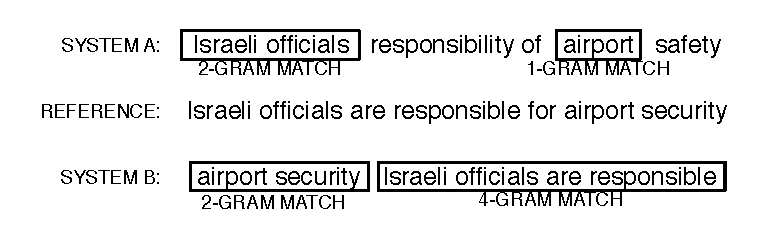
\includegraphics[scale=1.5]{bleu-example.pdf}
\begin{tabular}{c|c|c}
{\bf Metric} & \bf System A & \bf System B \\ \hline
precision (1gram) & 3/6 & 6/6 \\ \hline
precision (2gram) & 1/5 & 4/5 \\ \hline
precision (3gram) & 0/4 & 2/4 \\ \hline
precision (4gram) & 0/3 & 1/3  \\ \hline
brevity penalty   & 6/7 & 6/7  \\ \hline 
{\sc bleu} &  0\% & 52\%  \\ \hline
\end{tabular}
\end{center}
\end{figure}


In short, the BLEU score calculation is an automatic evaluation of how similar two copora are. In the current experiments we are comparing the predicted target sequences with the gold standard. The BLEU score of 100 means the two copora are identical, and the BLEU score of 0 means the two copora are completely distinct from each other.

\begin{exe}
\ex Gold-Standard = English sentences in (\ref{GLOSStoENTest}) = English sentences in (\ref{GDtoENTest})
\end{exe}
Note that the gold-standard is the same because they are the same English sentences in the 3-tuples samples. Then the two sets of predicted English sentences are evaluated, yielding two BLEU scores.  

\begin{exe}
\ex Scores: \\
 \begin{xlist}
	\ex Score\textsubscript{GLOSStoEN} = BLEU(Gold-Standard, Predictions\textsubscript{GLOSStoEN}) \\
	\ex Score\textsubscript{GDtoEN} = BLEU(Gold-Standard, Predictions\textsubscript{GDtoEN}) \\
 \end{xlist}
\end{exe}
This procedure of splitting the data into three sub-sets, training the models, and evaluating the models is executed for ten times.

\subsection{Result} \label{gdglen_results}
After ten rounds of repeated random sub-sampling validation, ten pairs of scores of the two models are generated, as shown in the following table.
% !Rnw root = cake_chapter.Rnw
% latex table generated in R 3.4.4 by xtable 1.8-2 package
% Tue Apr 10 20:51:14 2018
\begin{table}[ht]
\centering
\begin{tabular}{lcc}
  \hline
Round & Gaelic (Baseline) & GLOSS \\ 
  \hline
0 & 17.29 & 18.39 \\ 
  1 & 16.42 & 18.00 \\ 
  2 & 15.29 & 16.02 \\ 
  3 & 15.97 & 20.22 \\ 
  4 & 17.79 & 19.02 \\ 
  5 & 16.73 & 15.53 \\ 
  6 & 17.11 & 18.00 \\ 
  7 & 16.37 & 20.08 \\ 
  8 & 15.93 & 15.82 \\ 
  9 & 16.99 & 15.93 \\ 
   \hline
Mean & 16.59 & 17.70 \\ 
   \hline
\end{tabular}
\caption{BLEU scores of Model\textsubscript{GDtoEN} and Model\textsubscript{GLOSStoEn}} 
\label{Table:GLOSS}
\end{table}
The average score of the Models\textsubscript{GLOSStoEN} is only sightly higher than the average score of the Models\textsubscript{GDtoEN}.
Also, after doing a paired T-test, the difference between the two types of models is not attested
(M\textsubscript{GDToEn}=16.59, SD\textsubscript{GDToEn}=0.74; M\textsubscript{GLOSStoEN}=17.70, SD\textsubscript{GLOSStoEN}=1.78; t(9)=1.97, p=0.080)

\subsection{Summary}
The ultimate practical goal of the dissertation is to use glossing data to develop better machine translation systems. Here \textit{better} means to be better than a baseline system, which is the machine translation system trained with Gaelic-to-English translation samples. The models in (\ref{ModelGDToEN}) are the baseline systems, and their scores are in the Gaelic column of table (\ref{Table:GLOSS}). These are the target scores that we aims to outperform. The experiment above is the first attempt to improve that scores by using the \textit{gloss treatment}, in which the Gaelic sentences are replaced with gloss lines.  However, the result shows that this \textit{gloss treatment} is not effective as the scores of the gloss models are not statistically higher than the baseline Gaelic-to-English models. 

\subsection{Discussion}
It is assumed that the performances of the machine translation systems are correlated with the quality of the representation of meanings in the source sequences. Better representations of meanings yield better machine translation systems. Given the results in (\ref{gdglen_results}) that the gloss models are not better than the Gaelic models, it is concluded that glosses and natural languages are equally good in terms of representing meanings. The strong version of the Gloss-helps hypothesis does not hold.

There are several remarks that need to make for the current result. First, the result falsifies the point of view about glosses in chapter (\ref{chap:gloss}) that the gloss line is a golden semantic representation hand-crafted by linguists.
It turns that this artificial language, the gloss lines, is only marginal better than Gaelic, as the mean BLEU score of the gloss treatment is slightly higher than that of the baseline systems. This can be viewed as an evidence of language evolution.
The written form of a natural language is actually already optimized for representing semantics to the same degree of gloss line representations.
Second, if we want to actually apply the gloss treatment to translate a Gaelic sentence to English, we encounter an immediate problem. The actual source sequence is a Gaelic sentence, while the required source sequence for the gloss treatment is a gloss line. The auto-glosser described in chapter (\ref{chap:gloss}) may convert the Gaelic sentence to a gloss line, but the conversion is not perfect at all. Given this, even if the gloss treatment should work, it is not practical unless we may convert Gaelic sentence to gloss line perfectly.      

We may now combine Gaelic and Gloss sentences as the training data to test the weak version of the Gloss-helps hypothesis. The experiments and results are reported in the next chapter.
%%%%%%%%%%%%%%%%%%%%%%%%%%%%%%%%%%%%%%%%%%%%%%%%%%%%%%%%%%%%%%%%%%%%%%%%%%%%%%%%%%%%%%%%%%%
\chapter{Combining Gaelic Words with Glosses}\label{chap:cake2}
\section{Introduction}
In the previous chapter, we attempt to build a system by using the \textit{gloss treatment} to outperform the baseline system. It turns that using gloss line solely is not effective enough to improve the system. However, this result does not falsify the gloss-helps hypothesis; instead, it indicates that combination of the gloss line data and the Gaelic sentence data is necessary. In other words, the questions now are: 
\begin{exe}
	\ex 
	\begin{xlist}
		\ex Does adding the gloss data into the Gaelic data will improve the translation system? 
		\ex If yes, what are the right ways of blending these two types of meaning representations together? 
	\end{xlist}	
\end{exe}

This section reports various ways of combining the gloss line data and the Gaelic sentence data, and the experiments and their results using these different treatments. Critically, a specific way of combining Gloss data and Gaelic date (termed as `\textit{Parallel-Partial}' treatment) boosts the performance significantly. The model trained with this specially arranged training data also significantly outperforms Google's Gaelic-to-English translation system.

In this section, I will first describe the most effective treatment, termed as `\textit{Parallel-Partial}' treatment, and the results, and then I will report the experiments done with other relevant logical treatments (i.e. other ways of combining glossing data and Gaelic data). 

\subsection{The Underlying Heuristics}\label{heuristics}
At a high level, neural net sequence to sequence learning algorithm is to learn how to map a high-dimension space to another high-dimension space. In the settings of machine translation, each dot in the high-dimension space is a meaning representation. Linking one dot to another dot is converting one meaning representation to another, yielding the effect of translation. Given this heuristics, we may just feed the machine with all the available meaning mappings. Given the assumption that the gloss lines are linguistically guided meaning representations, they are suitable training data for building machine translation systems. Specially, with the gloss data, we let the machine to learn the following mappings:

\begin{exe}
	\ex Mappings Learned in the ParaPart treatment
	\begin{xlist}
		\ex Gaelic sentences $\rightarrow$ English sentences
		\ex Gloss lines $\rightarrow$ English sentences
		\ex Gloss lines $\rightarrow$ Gaelic sentences
		\ex Gloss items $\rightarrow$ Gaelic words
	\end{xlist}	
\end{exe}    

\section{The `Parallel-Partial' Treatment Outperforms Any Other Treatments and the Baseline Significantly}

\subsection{Related work}
The Parallel-Partial treatment section may be viewed as a form of multi-task Sequence to Sequence Learning \citep{luong2015multi}. Specifically, the parallel part of the treatment is very similar to the data manipulation used in building multi-language translation systems \citep{google_zero_shot}.  

\subsection{Data Preprocessing Using the Parallel-Partial Treatment}
The Parallel-Partial treatment uses the training and validation data of the baseline system and that of the gloss treatment system.  
The training and validation data of the baseline system are pairs of a Gaelic sentence and a English sentences (see (\ref{GDtoENTrain}) and (\ref{GDtoENVal}) ), 
and the data of the gloss treatment are pairs of a gloss line and a English sentences (see (\ref{GLOSStoENTrain}) and (\ref{GLOSStoENVal}). 
These two groups of data are combined in a parallel manner in the current treatment. Now the size of training set and validation set is doubled. In the baseline system and the gloss treatment system, we have 6,388 samples in the training set and 1,000 samples in the validation set. The current treatment has 12,776 samples in the training set and 2,000 samples in the validation set. This is the \textit{parallel} part of the treatment. 

Additionally, I utilize the alignment property between the Gaelic word and the gloss to further build pairs of a Gaelic word and a gloss. These pairs are also included into the training set and validation set of the current treatment. This is the \textit{partial} part of the treatment.   

For concreteness, consider the following interlinear glossed text: 
\begin{exe}  
\ex \gll    Tha a athair nas sine na a mh\`athair.\\  
            be.pres 3sm.poss father comp old.cmpr comp 3sm.poss mother\\  
    \glt    `His father is older than his mother.'  
\end{exe}

With the interlinear glossed text, the parallel treatment will generate two pairs of samples:

\begin{exe}
	\ex
	\begin{xlist}
		\ex Gaelic to English: \\<``Tha a athair nas sine na a mh\`athair'', ``His father is older than his mother.''>
		\ex Gloss to English: \\<``be.pres 3sm.poss father comp old.cmpr comp 3sm.poss mother'', ``His father is older than his mother''>
	\end{xlist}
\end{exe}

The partial treatment then generates pairs of a Gaelic word and a gloss token: 
\begin{exe}
	\ex
	\begin{xlist}
		\ex <``Tha'', ``be.pres''>
		\ex <``a'', ``3sm.poss''>
		\ex <``athair'', ``father''>
		\ex <``nas'', ``comp''>
		\ex <``sine'', ``old.cmpr''>
		\ex <``na'', ``comp''>
		\ex <``a'', ``3sm.poss''>
		\ex <``mh\`athair'', ``mother''>
	\end{xlist}
\end{exe}

\subsection{Results of the Parallel-Partial Treatment}

Critically, the same technical settings and the same test sets in the previous experiments are used, and the same procedures are executed. The same split of the original IGTs is used, so as long as it is the same round, the training, validation and test are the same set of IGTs. The only difference is that now the training and validation IGT data are treated with the Parallel-Partial treatment. The result show that the Parallel-Partial treatment has a tremendous effect in improving the baseline system. 

% !Rnw root = cake_chapter.Rnw
% latex table generated in R 3.4.4 by xtable 1.8-2 package
% Tue Apr 10 20:51:14 2018
\begin{table}[ht]
\centering
\begin{tabular}{lcc}
  \hline
Round & Gaelic (Baseline) & ParaPart \\ 
  \hline
0 & 17.29 & 32.64 \\ 
  1 & 16.42 & 32.28 \\ 
  2 & 15.29 & 29.94 \\ 
  3 & 15.97 & 31.18 \\ 
  4 & 17.79 & 32.83 \\ 
  5 & 16.73 & 31.11 \\ 
  6 & 17.11 & 32.19 \\ 
  7 & 16.37 & 33.52 \\ 
  8 & 15.93 & 30.93 \\ 
  9 & 16.99 & 34.35 \\ 
   \hline
Mean & 16.59 & 32.10 \\ 
   \hline
\end{tabular}
\caption{BLEU scores of Model\textsubscript{GDtoEN} and Model\textsubscript{ParaParttoEn}} 
\label{Table:ParaPart}
\end{table}
The first and the second columns are BLUE scores of the baseline systems and the systems with the Parallel-Partial treatment respectively. The latter is significantly better than the former
(M\textsubscript{GDToEn}=16.59, SD\textsubscript{GDToEn}=0.74; M\textsubscript{ParaPart}=32.10, SD\textsubscript{ParaPart}=1.33; t(9)=48.95, p<0.01).
The comparison of the average BLUE scores of the groups of systems shows that the Parallel-Partial treatment improves the performance of the baseline system for 93 percent.
%(M\textsubscript{GDToEn}=16.59, SD\textsubscript{GDToEn}=0.74; M\textsubscript{ParaPart}=32.10, SD\textsubscript{ParaPart}=1.33,; t(9)=48.95, p<0.010.000).
\subsubsection{Discussion}
With the ParaPart treatment, the baseline systems are improved for more than 93 percent. This result suggest the validity of our heuristics in section \ref{heuristics}, and provide strong evidence for the gloss-helps hypothesis in (\ref{hypothesis}).     


%%%%%%%%%%%%%%%%%%%%%%%%%%%%%%%%%%%%
\section{Other Possible Treatments}
This section reports other possible ways of blending the Gaelic sentences and gloss lines. However, all of these treatments are not as effective as the Parallel-Partial treatment. Again, the same procedure and the same test datasets are used across all the experiments.    

\subsection{The Parallel Treatment}\label{treatment:Para}
\subsubsection{Method of the Parallel Treatment}
The Parallel treatment is using the parallel part of the Parallel-Partial treatment without exploiting the alignment properties of gloss lines.
It is expected that this treatment will improve the baseline systems but will not be as effective as the Parallel-Partial treatment.

With this treatment, a chunk of interlinear glossed text is split into two pairs. For example, the chunk of interlinear glossed text in (\ref{igt}) becomes two samples in (\ref{sample_pair}): 
\begin{exe} 
\ex \label{igt}
	\gll    Tha a athair nas sine na a mh\`athair.\\  
            be.pres 3sm.poss father comp old.cmpr comp 3sm.poss mother \\
    \glt    `His father is older than his mother.'  
\end{exe}


\begin{exe} 
	\ex \label{sample_pair}
	\begin{xlist}
		\ex Gaelic to English: \\<``Tha a athair nas sine na a mh\`athair'', ``His father is older than his mother.''>
		\ex Gloss to English: \\<``be.pres 3sm.poss father comp old.cmpr comp 3sm.poss mother'', ``His father is older than his mother''>
	\end{xlist}
\end{exe}

\subsubsection{Results of the Parallel Treatment}\label{treatment:Para_result}
The experiments had our expected results. 
% !Rnw root = cake_chapter.Rnw
% latex table generated in R 3.4.4 by xtable 1.8-2 package
% Tue Apr 10 20:51:14 2018
\begin{table}[ht]
\centering
\begin{tabular}{lcc}
  \hline
Round & Gaelic (Baseline) & Para \\ 
  \hline
0 & 17.29 & 25.42 \\ 
  1 & 16.42 & 25.32 \\ 
  2 & 15.29 & 20.72 \\ 
  3 & 15.97 & 22.22 \\ 
  4 & 17.79 & 24.27 \\ 
  5 & 16.73 & 24.55 \\ 
  6 & 17.11 & 27.03 \\ 
  7 & 16.37 & 25.34 \\ 
  8 & 15.93 & 24.24 \\ 
  9 & 16.99 & 25.96 \\ 
   \hline
Mean & 16.59 & 24.51 \\ 
   \hline
\end{tabular}
\caption{BLEU scores of Model\textsubscript{GDtoEN} and Model\textsubscript{ParatoEn}} 
\label{Table:Para}
\end{table}The table in (\ref{Table:Para}) compares the performances of this treatment and the baseline. Critically, the Parallel treatment is effective in improving the baseline systems (M\textsubscript{GDToEn}=16.59, SD\textsubscript{GDToEn}=0.74; M\textsubscript{Para}=24.51, SD\textsubscript{Para}=1.84; t(9)=17.50, p < 0.01). 
% !Rnw root = cake_chapter.Rnw
%GDParaParaPart1_table.Rnw does NOT print out anything but just load the sexpr variables 
However, the best treatment (i.e. the Parallel-Partial treatment) is still far better than this Parallel treatment 
(M\textsubscript{Para}=24.51, SD\textsubscript{Para}=1.84; M\textsubscript{ParaPart}=32.10, SD\textsubscript{ParaPart}=1.33; t(9)=18.73, p < 0.01 ).
% !Rnw root = cake_chapter.Rnw
% latex table generated in R 3.4.4 by xtable 1.8-2 package
% Tue Apr 10 20:51:14 2018
\begin{table}[ht]
\centering
\begin{tabular}{lccc}
  \hline
Round & Gaelic (Baseline) & Para & ParaPart \\ 
  \hline
0 & 17.29 & 25.42 & 32.64 \\ 
  1 & 16.42 & 25.32 & 32.28 \\ 
  2 & 15.29 & 20.72 & 29.94 \\ 
  3 & 15.97 & 22.22 & 31.18 \\ 
  4 & 17.79 & 24.27 & 32.83 \\ 
  5 & 16.73 & 24.55 & 31.11 \\ 
  6 & 17.11 & 27.03 & 32.19 \\ 
  7 & 16.37 & 25.34 & 33.52 \\ 
  8 & 15.93 & 24.24 & 30.93 \\ 
  9 & 16.99 & 25.96 & 34.35 \\ 
   \hline
Mean & 16.59 & 24.51 & 32.10 \\ 
   \hline
\end{tabular}
\caption{BLEU scores of Model\textsubscript{GDtoEN}, Model\textsubscript{ParatoEN} and Model\textsubscript{ParaParttoEN} } 
\label{Table:Concating}
\end{table}
Critically, the comparison between the Parallel-Partial treatment and current Parallel-Only treatment shows the effectiveness of the word-gloss alignments. Our conjecture on the effectiveness is that with the pairs of a gloss item and a Gaelic word present in the training data, the burden of the attention algorithm \citep{bahdanau2014neural} is largely alleviated. In other words, instead of asking the attention algorithm to estimate what to attend to, we explicitly teach the machine the alignment between the Gaelic word and the corresponding gloss. 

\subsection{Interleaving Gaelic Words and Gloss Items And Concating them}\label{treatment:InterleavingAndConCat}
\subsubsection{Method of the Interleaving Treatment}
Instead of putting the pairs of a Gaelic sentence and a English sentences and the pairs of a gloss line and a English sentence in a parallel manner, we may just literally blend a Gaelic sentence and a gloss line by interleaving them\footnote{\citet{ccg_target_seq} incorporate the Categorial grammar parse tags into natural sentences by interleaving the tags and the words.}. Consider the following example:

\begin{exe} 
\ex 
	\begin{xlist}
	\ex \label{ex_interleave:in}
		\gll	 Tha a athair nas sine na a mh\`athair.\\  
     		     be.pres 3sm.poss father comp old.cmpr comp 3sm.poss mother \\
    	\glt    `His father is older than his mother.'  

    \ex \label{ex_interleave:out} <``Tha be.pres a 3sm.poss athair father nas comp sine old.cmpr na comp a 3sm.poss mh\`athair mother'', ``His father is older than his mother''>
    \end{xlist}
\end{exe}

Given the chuck of interlinear glossed text data in (\ref{ex_interleave:in}), the Interleaving treatment generates the sample in (\ref{ex_interleave:out}).  

This way of blending gloss lines and Gaelic sentences may add useful information into the training data; however, the downside of this method is to increase the length our samples on the source sequence side. In neural net machine learning, the longer the sequences are, the harder it is to preserve all the information. So, this treatment may not be effective. 


The results are given in the following table. 
% !Rnw root = cake_chapter.Rnw
% latex table generated in R 3.4.4 by xtable 1.8-2 package
% Tue Apr 10 20:51:14 2018
\begin{table}[ht]
\centering
\begin{tabular}{lcc}
  \hline
Round & Gaelic (Baseline) & interleavingGdGLOSS \\ 
  \hline
0 & 17.29 & 13.67 \\ 
  1 & 16.42 & 12.49 \\ 
  2 & 15.29 & 11.01 \\ 
  3 & 15.97 & 12.33 \\ 
  4 & 17.79 & 12.56 \\ 
  5 & 16.73 & 12.13 \\ 
  6 & 17.11 & 11.55 \\ 
  7 & 16.37 & 12.78 \\ 
  8 & 15.93 & 12.43 \\ 
  9 & 16.99 & 11.65 \\ 
   \hline
Mean & 16.59 & 12.26 \\ 
   \hline
\end{tabular}
\caption{BLEU scores of Model\textsubscript{GDtoEN} and Model\textsubscript{interleavingGdGLOSStoEn}} 
\label{Table:interleavingGdGLOSS}
\end{table}\newline
It turns out this treatment has a significant negative effect
(M\textsubscript{GDToEn}=16.59, SD\textsubscript{GDToEn}=0.74; M\textsubscript{interleavingGdGLOSS}=12.26, SD\textsubscript{interleavingGdGLOSS}=0.74,; t(9)=-17.06, p=0.000). This is not the right way of incorporating gloss line data. 


\subsubsection{Method of Concating Gaelic Words and Gloss Words }\label{treatment:Concating}
A quick and close amendment of the Interleaving approach is to concatenate the aligned Gaelic word and gloss item as a single token. Given the same chunk of interlinear glossed text data, this treatment generates the following sample:

\begin{exe} 
\ex 
	\begin{xlist}
	\ex 
		\gll	 Tha a athair nas sine na a mh\`athair.\\  
     		     be.pres 3sm.poss father comp old.cmpr comp 3sm.poss mother \\
    	\glt    `His father is older than his mother.'  

    \ex <``Tha\_be.pres a\_3sm.poss athair\_father nas\_comp sine\_old.cmpr na\_comp a\_3sm.poss mh\`athair\_mother'', ``His father is older than his mother''>
    \end{xlist}
\end{exe}

Concating words and glosses does solve the long sequence problem; however, it causes the sparse data problem. In this arrangement, the number of the types of tokens is increased; the number of tokens of each type is decreased. Thus all the samples are put in a larger space. So, the treatment may not be effective either. 

\subsubsection{Results of Concating Gaelic Words and Gloss Words}
The performances of this treatment is given in the following table.
% !Rnw root = cake_chapter.Rnw
% latex table generated in R 3.4.4 by xtable 1.8-2 package
% Tue Apr 10 20:51:14 2018
\begin{table}[ht]
\centering
\begin{tabular}{lcc}
  \hline
Round & Gaelic (Baseline) & ConcatGLOSSGaelic \\ 
  \hline
0 & 17.29 & 15.42 \\ 
  1 & 16.42 & 14.31 \\ 
  2 & 15.29 & 15.38 \\ 
  3 & 15.97 & 14.18 \\ 
  4 & 17.79 & 18.63 \\ 
  5 & 16.73 & 14.89 \\ 
  6 & 17.11 & 15.16 \\ 
  7 & 16.37 & 15.20 \\ 
  8 & 15.93 & 15.50 \\ 
  9 & 16.99 & 15.72 \\ 
   \hline
Mean & 16.59 & 15.44 \\ 
   \hline
\end{tabular}
\caption{BLEU scores of Model\textsubscript{GDtoEN} and Model\textsubscript{ConcatGLOSSGaelictoEn} } 
\label{Table:Concating}
\end{table}\newline
The result shows that this treatment hurts the baseline systems instead of improving them (M\textsubscript{GDToEn}=16.59, SD\textsubscript{GDToEn}=0.74; M\textsubscript{ConcatGLOSSGaelic}=15.44, SD\textsubscript{ConcatGLOSSGaelic}=1.23,; t(9)=-3.64, p=0.010).

%%%%%%%%%%
\subsection{Hybrid: Gaelic or Gloss}
\subsubsection{Method of Hybrid}
The Hybrid treatment aims to reduce the potential lexical ambiguity. A Gaelic word may maps to multiple gloss, and a glosses may maps to multiple Gaelic words. Let's assume a toy chunk of interlinear glossed text data (a one-word sentence): 

\begin{exe} 
\ex 
	\gll	 Gaelic\_word\\  
     		 Gloss\_item \\
    \glt    English translation  
\end{exe} 

Now we aim to build a single sample that is either <Gaelic\_word, English translation > or <Gloss\_item, English translation >. The criterion is which one, the Gaelic word or the gloss item, is less ambiguous. 
The less ambiguous one is the winner. For example, if the Gaelic word is potentially mapped to 10 glosses and if the gloss item is potentially mapped 2 Gaelic word, then <Gloss\_item, English translation> is chosen; other the other hand if the ambiguity situation is reverted, then <Gaelic\_word, English translation > is chosen. 
However, when the situation is tight (i.e. both the Gaelic word and gloss item are equally ambiguous), a default setting is needed to be chosen. The choices of the default setting split this single treatment into two treatments: default as Gaelic or default as gloss.

The following is an example of the hybrid treatment:

\begin{exe}
\ex
	\gll tha nathairichean a`chuir an t-eagal orm\\
		 be.pres snake.vn put det fear on.1s\\
	\glt `Snakes frighten me' 
\end{exe} 

\subsubsection{Result of Hybrid}    
% !Rnw root = cake_chapter.Rnw
% latex table generated in R 3.4.4 by xtable 1.8-2 package
% Tue Apr 10 20:51:14 2018
\begin{table}[ht]
\centering
\begin{tabular}{lcc}
  \hline
Round & Gaelic (Baseline) & HybridDefaultAsGaelic \\ 
  \hline
0 & 17.29 & 9.44 \\ 
  1 & 16.42 & 9.07 \\ 
  2 & 15.29 & 7.69 \\ 
  3 & 15.97 & 9.12 \\ 
  4 & 17.79 & 9.08 \\ 
  5 & 16.73 & 10.45 \\ 
  6 & 17.11 & 8.62 \\ 
  7 & 16.37 & 10.00 \\ 
  8 & 15.93 & 10.52 \\ 
  9 & 16.99 & 8.46 \\ 
   \hline
Mean & 16.59 & 9.24 \\ 
   \hline
\end{tabular}
\caption{BLEU scores of Model\textsubscript{GDtoEN} and Model\textsubscript{HybridDefaultAsGaelictoEn}} 
\label{Table:HybridDefaultAsGaelic}
\end{table}When the default setting is the Gaelic word, the performances are significantly worse than than the baseline systems, as shown in table (\ref{Table:HybridDefaultAsGaelic}).  
(M\textsubscript{GDToEn}=16.59, SD\textsubscript{GDToEn}=0.74; M\textsubscript{ReplacingGaelic}=9.24, SD\textsubscript{ReplacingGaelic}=0.89,; t(9)=-21.03, p < 0.01).



% !Rnw root = cake_chapter.Rnw
% latex table generated in R 3.4.4 by xtable 1.8-2 package
% Tue Apr 10 20:51:14 2018
\begin{table}[ht]
\centering
\begin{tabular}{lcc}
  \hline
Round & Gaelic (Baseline) & HybridDefaultAsGLOSS \\ 
  \hline
0 & 17.29 & 15.95 \\ 
  1 & 16.42 & 15.60 \\ 
  2 & 15.29 & 14.15 \\ 
  3 & 15.97 & 14.72 \\ 
  4 & 17.79 & 15.74 \\ 
  5 & 16.73 & 14.88 \\ 
  6 & 17.11 & 14.45 \\ 
  7 & 16.37 & 16.41 \\ 
  8 & 15.93 & 15.15 \\ 
  9 & 16.99 & 17.61 \\ 
   \hline
Mean & 16.59 & 15.47 \\ 
   \hline
\end{tabular}
\caption{BLEU scores of Model\textsubscript{GDtoEN} and Model\textsubscript{HybridDefaultAsGLOSS}} 
\label{Table:HybridDefaultAsGLOSS}
\end{table}When the default setting is the Gaelic word, the performances are sightly worse than than the baseline systems, as shown in table (\ref{Table:HybridDefaultAsGLOSS}).
(M\textsubscript{GDToEn}=16.59, SD\textsubscript{GDToEn}=0.74; M\textsubscript{ReplacingGaelic}=15.47, SD\textsubscript{ReplacingGaelic}=1.03,; t(9)=-3.67, p < 0.01 ).


\section{Summary and Conclusion}
The chapter reports machine translation experiments that aims to find how the gloss line information can improve the performance of the baseline Gaelic-to-English translation systems. It is found that the Parallel-Partial is highly effective. The complete BLEU scores of various treatments are given in the following table.

%\begin{adjustbox}{angle=90} 
% latex table generated in R 3.4.4 by xtable 1.8-2 package
% Tue Apr 10 20:51:14 2018
\begin{table}[ht]
\centering
\begin{tabular}{lrrrrrrrr}
  \hline
\begin{sideways} Round \end{sideways} & \begin{sideways} Baseline \end{sideways} & \begin{sideways} GLOSS \end{sideways} & \begin{sideways} ParaPart \end{sideways} & \begin{sideways} Para \end{sideways} & \begin{sideways} Interleaving \end{sideways} & \begin{sideways} Concat \end{sideways} & \begin{sideways} HybrGaelic \end{sideways} & \begin{sideways} HybrGLOSS \end{sideways} \\ 
  \hline
0 & 17.29 & 18.39 & 32.64 & 25.42 & 13.67 & 15.42 & 9.44 & 15.95 \\ 
  1 & 16.42 & 18.00 & 32.28 & 25.32 & 12.49 & 14.31 & 9.07 & 15.60 \\ 
  2 & 15.29 & 16.02 & 29.94 & 20.72 & 11.01 & 15.38 & 7.69 & 14.15 \\ 
  3 & 15.97 & 20.22 & 31.18 & 22.22 & 12.33 & 14.18 & 9.12 & 14.72 \\ 
  4 & 17.79 & 19.02 & 32.83 & 24.27 & 12.56 & 18.63 & 9.08 & 15.74 \\ 
  5 & 16.73 & 15.53 & 31.11 & 24.55 & 12.13 & 14.89 & 10.45 & 14.88 \\ 
  6 & 17.11 & 18.00 & 32.19 & 27.03 & 11.55 & 15.16 & 8.62 & 14.45 \\ 
  7 & 16.37 & 20.08 & 33.52 & 25.34 & 12.78 & 15.20 & 10.00 & 16.41 \\ 
  8 & 15.93 & 15.82 & 30.93 & 24.24 & 12.43 & 15.50 & 10.52 & 15.15 \\ 
  9 & 16.99 & 15.93 & 34.35 & 25.96 & 11.65 & 15.72 & 8.46 & 17.61 \\ 
   \hline
Mean & 16.59 & 17.70 & 32.10 & 24.51 & 12.26 & 15.44 & 9.24 & 15.47 \\ 
   \hline
\end{tabular}
\caption{BLEU scores of the treatments} 
\label{table:complete_table}
\end{table}%\end{adjustbox}

The aim of chapter is to report and document how the experiments are done and what the results are. This is merely reporting the linguist and non-linguistic facts. The implications and relevant works in the literature will be discussed in the next chapter.   


(
Hi Mike: 
The current chapter reports the what are done and how (i.e. the fact);
the next chapter I will discuss the why questions, and discuss similar works in the literature.  

)
% \subsection{literature}

% what about \ref{Table:interleavingGdGLOSS} \ref{table:complete_table}
% Linguistics-informed MT: \citep{sennrich2016linguistic}\\ 

% Multi-task Sequence to Sequence Learning: \citep{luong2015multi}\\
% what is Multi-task learning:  \citep{Overview_Multi-Task_Learning}\\
% add ccc to target seq: \citep{ccg_target_seq}\\
% google zero shot: \citep{google_zero_shot}\\
\chapter{Interlinear Glossed Text Data In Other Languages}
\label{chap:gloss_in_other_languages}

To run the same experiments on Online Database of Interlinear Text \citep{ODIN, Xia2016} to show that incorporating gloss information works effectively across different languages.  
\chapter{Implications on Theoretical Linguistics and Natural Language Processing}
\label{chap:Implications}

Cite Pater 
Pater 2017: Generative linguistics and neural networks at 60: foundation, friction and fusion
\chapter{Conclusion}
Conclusion


\bibliographystyle{te}

\bibliography{ref}

\end{document}
